%!TEX root = ../main.tex
\chapter{An Unified Efficient Particle Physics Framework}
\label{new_lipmini}

Programming for homogeneous platforms poses a series of challenges not faced when coding parallel applications due to the shared memory paradigm. In this context, the data is always easily accessible when coding, as the different memory bank accesses are managed by the compiler and hardware. Data dependencies and races still need to be managed by the programmer, which may required a significant level of expertise. To efficiently use the computational resources, dealing with problems such as false sharing or efficient cache usage, the programmer must have an advanced expertise on both the coding and architectural details of homogeneous platforms.

Since an heterogeneous platform is a distributed memory environment, where the CPUs shared the memory with each other but not with the hardware accelerators, a series of new challenges arise. All communications of data between CPU and accelerator must be explicitly coded by the programmer, and has an added latency associated. The balance of the work for each computing device to process becomes harder as it must take into account the data transfers and different characteristics of the devices.

Each different hardware accelerator has its own architectural design principles, as show in section \ref{hardware}, which constrain the way they are programmed and the characteristics that both the algorithm and the code must have to efficiently use the computational resources. This implies that the programmer must be able to learn the hardware intrinsic characteristics and adapt to a new programming paradigm. Even for experienced programmers, adapting current applications to run on heterogeneous platforms may be infeasible without redesigning all major algorithms, as opposed to code a new application specifically for these platforms. This issue has an higher impact on legacy code.

Scientists are usually self-taught programmers that only consider coding as a necessary tool to perform their research. Several studies, referred in section \ref{motivation}, identified a set of problems with scientists coding practices and scientific computing. Most of their code is in constant development, up to decades long, only adding or changing functionalities in each iteration, not considering any software engineering principles and not adapting the code to the changes in hardware. The few that worry about performance attempt to address the code regions that they think are the bottleneck, not knowing of the existence of profiling tools and even compiler optimisations.

Since most scientists develop applications with the help of specialised frameworks of their research field, they expect them to be efficient, by resorting to parallelisation or other techniques. However, the bottleneck is often on the scientists code rather than in the framework, and these tools are not designed to automatically extract parallelism from their code.

Scientists usually do not have any training for programming efficient applications for homogeneous systems or cluster environments, as programming is just a necessity for their field of research. They are even more reluctant to learn the new programming paradigms required to work with hardware accelerators on heterogeneous platforms. With this in mind, several automatically parallelisation frameworks for these systems were developed by computer scientists, as presented in subsection \ref{distributed_mem}.

These general purpose frameworks usually have a steep learning curve, even for computer scientists. One significant setback of these frameworks is that, even if it is not explicitly required, the application must be designed to the framework characteristics, rather than the framework adapt to the application. As scientists are usually reluctant to redesign the very complex legacy code, which is difficult for computer scientists to understand without the expertise of the science field, an integration with these frameworks is infeasible. This problem also applies to the most of the external libraries used by these applications, as their functions are not coded to run on hardware accelerators and adapting the source code may not be possible.

Even though, scientists are not willing to endure the steep learning curve of these frameworks to integrate with future applications, and do not want to code two versions of the core algorithms to run on the CPU and accelerator. Their complexity and the lack of guarantees to that they will increase the code performance, due to poor implementation or algorithm characteristics, puts the scientists further away from these frameworks. Also, they attempt to have few dependencies of an application with external libraries, as the external tools are not guaranteed to be supported through the application lifetime.

The existence of general purpose automatically parallelisation frameworks is useful, specially for computer scientists, but the scientific community lacks frameworks that both address the intrinsics of their scientific field, in which scientists can trust and rely, and the efficient usage of the computational resources, on both homogeneous and heterogeneous platforms. Frameworks such as these sacrifice the abstraction to interact with any scientific field, but are more adapted to the scientific problem that is addressed. A lower abstraction level leads to an easy interaction of the scientist with the tool (and even abstract them of any parallelisation complexities) and increases the computational efficiency of the code when compared with general purpose frameworks, as the main bottlenecks are usually known \textit{a priori} and the framework is designed around their characteristics. The development of such frameworks may lead to a better interface of computer scientists and researchers, causing and improvement of their codes with the implementation of software engineering concept, increasing the quality of the research.

\section{The LipMiniAnalysis Skeleton Library}
\label{lipminianalysis}

The LipCbrAnalysis was a skeleton developed by two researchers of LIP in 2005, with the purpose of aiding the development of data analysis applications within the research group. Initially it served as an interface for dealing with the I/O of the data, transforming it from the format supported by ROOT at the time to variables in the global memory of the skeleton. All other standard functions needed for the analysis had their prototypes declared, but it was the programmers job to code them to his needs, knowing that the required data for each event was on memory.

Along the years the code was successively iterated to add support for new data file formats, physics functionalities, and general features, such as the support for passing options and arguments to the executable. Some of the functions that the programmer needed to code were now fully implemented, with the option of being override by the user.

The LipMiniAnalysis is the latest development iteration on a production environment. It discarded outdated features that were no longer necessary, and reads the new Mini Ntuple data format, hence its name. It is not a standard ROOT data format, but rather a set of events that suffered some preprocessing to improve the quality of the data and filter events that do not show any interesting physics.

Figure \ref{fig:lipmini} presents the structure of LipMiniAnalysis, where all sections marked with a \textbf{*} need to be coded by the programmer. When the application starts it sets the default values for all control information needed by the event filtering and reconstruction. The \textit{Set User Values} section allows for the user to set its own control parameters, for both information defined by \textit{Set Default Values}, overwriting the existing configuration, and parameters not set yet. The \textit{Get Command Line Options} section is responsible for defining and interpreting the options defined by the user when starting the executable. It is partially defined with standard options for every analysis, such as the definition of the systematics file and output directory, but the programmer can add new options as needed. The systematics parameters are automatically configured based on the input systematics file, so no user interaction is necessary. The preparation of both the input and output files is done automatically, but the declaration of the histogram vectors must be coded by the programmer, as it depends on the event type, filtering and reconstruction techniques applied.

\begin{figure}[!htp]
	\begin{center}
		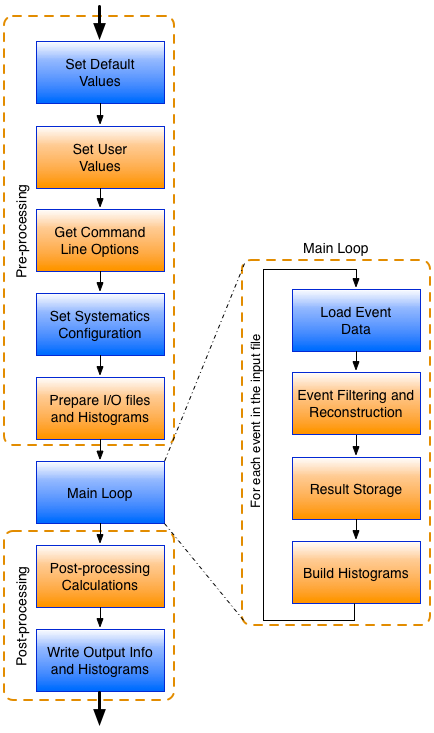
\includegraphics[scale=0.5]{imgs/lipminianalysis.png}
		\caption{Schematic representation LipMiniAnalysis skeleton structure. The \textbf{*} mark represents the sections of the skeleton that the programmer must code.}
		\label{fig:lipmini}
	\end{center}
\end{figure}

The \textit{Main Loop} is responsible for individually loading an event from the input file, apply the filters, reconstruct it if it passes the required filters, store the results, and build the histograms for each filter and final reconstruction. Only the event loading is automatic, so the programmer must code all remaining sections, as they vary among different analysis. The final post-processing also depends on the analysis, so it is not coded. Then, LipMiniAnalysis automatically writes all output information. Note that this is a logical structure of the code; in the current implementation most features are not properly organised and LipMiniAnalysis would have great benefits from a reorganisation of its structure, code-wise.

Studies presented in \cite{Msc:AMP,paperAMP} targeted the computational efficiency issues of a specific data analysis application of LIP, related to the reconstruction of the \ttH system. This data analysis was developed using the LipMiniAnalysis and, although the goal was to address only the inefficiencies of the data analysis itself, problems with the main data structure of the skeleton restricted the performance scalability, specially on heterogeneous platforms.

The LipMiniAnalysis was designed to store only one event in the application global memory for the \textit{Main Loop} to load and process. The data for an event is composed of hundreds of variables, from simple scalars to complex vectors of ROOT classes. With only a single event in memory, it is more difficult to create an efficient parallelisation with only the event reconstruction tasks, due to the low amount of work to balance, specially on distributed memory environments as it will require more communications through the application lifetime. With all events from an input data file on the application global memory, a more efficient parallelisation for both shared and distributed memory systems can be achieved. It would also help the implementation of automatic parallelisation in LipMiniAnalysis.

\section{The Proposed Framework}
\label{new_framework}

\itodo{especificaçao do que a nova framework tem de ter, design from scratch}

\subsection{Preliminary Tests and Prototypes}
\label{work_so_far}

\itodo{trabalho feito até agora, no aspecto que são protótipos a serem integrados na nova framework}
